\documentclass[conference, compsoc]{IEEEtran}
\usepackage[T1]{fontenc}
\usepackage{graphicx}

\begin{document}
\title{Deep Learning Lab 4}
\author{\IEEEauthorblockN{Hitesh Goyal - 19BAI1129,
\IEEEauthorblockA{
VIT Chennai, Tamil Nadu, India 600127\\
Email: hitesh.goyal2019@vitstudent.ac.in}
}}

\maketitle
\begin{abstract}
    Hyperparameter tuning is an important part of Deep Learning. It can help increase the accuracy of models and can also help realise how relevant a model is for the real world. Common problems in Deep Learning like overfitting are addressed with its help.
\end{abstract}

\section{Introduction}
In the fourth lab session, the aim is to use a library to tune the parameters of the deep neural network containing Convolutional Neural Networks. Convolutional Neural Network has the capability of filtering out spatial features while also reducing the dimensions (or size) of processing which can be essential when dealing with large amounts of data. It can be considered as a method of feature engineering done during training by the model itself.

\section{Dataset}
The dataset used for this lab is CIFAR10 dataset. It is a "tiny-image" dataset which contains a total of sixty thousand 32X32 images. There are a total of ten classes and each class has six thousand images. It is a well-balanced dataset. The classes which are labelled are - Airplane, Automobile, Bird, Cat, Deer, Dog, Frog, Horse, Ship and Truck.

\section{Methodology}
\subsection{Pre-training Tasks}
\subsubsection{Import Dataset}
CIFAR10 dataset can be directly imported from Tensorflow. One need not download it separately as Tensorflow has an inbuilt function which directly downloads it from a source.

\subsubsection{Split Data}
The dataset is split into three parts - training, validation and testing. The training data is used to train the network, the validation is used to tune it and the testing is used to finally evaluate the model's accuracy.

\subsubsection{Normalise Data}
Data normalisation is a very important step to make sure that the model trains in a faster and more effective way. It makes sure that the model is not biased towards certain features more than others. Normalising image data is fairly simple. Just dividing all the pixel values by 255 can make do the job.

\begin{figure}
    \centering
    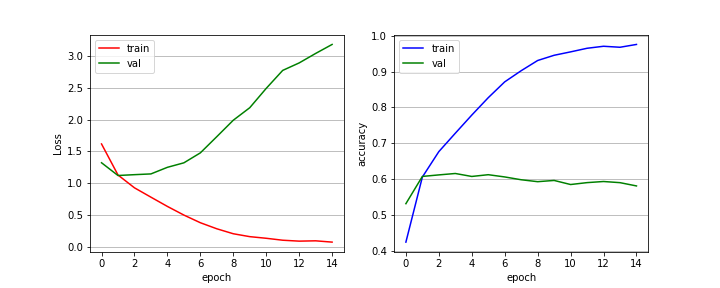
\includegraphics[scale=0.335]{../cifar10_training_val_no_dropout.png}
    \caption{Training and Validation accuracy of model with no regularisation}
    \label{fig:train_no_dropout}
\end{figure}

\begin{figure}
    \centering
    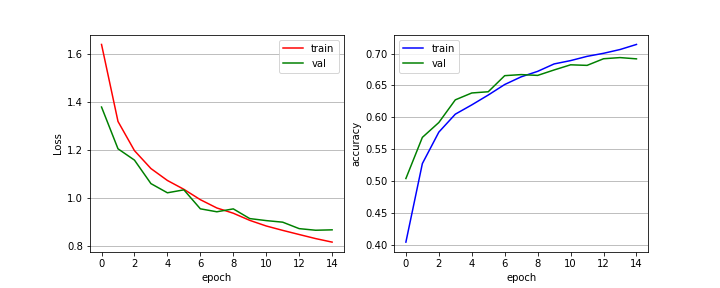
\includegraphics[scale=0.335]{../cifar10_training_val_with_dropout.png}
    \caption{Training and Validation accuracy of model with Dropout as a regulariser}
    \label{fig:train_with_dropout}
\end{figure}

\subsection{Model Building}
\subsubsection{Initial Model}
The first model is initialised with two convolution layers followed by a normal "Dense" layer. The model finally reaches its output layer. There is no regularisation used in this model. Upon training, it is seen that the model performs overfitting. This is identified by the gradual increase of training accuracy as opposed to a similar decrease in the validation. The accuracy and loss curve of the model can be seen in Figure \ref{fig:train_no_dropout}.


\subsubsection{Manual tuning}
To regularise this model, max pooling and dropout are used. max pooling is applied to both the convolution layers and dropout is applied after flattening the convolution layer and before passing it through the last hidden layer. It is observed that the accuracy on training and validation both increase at about the same rate. The issue with this model is that the accuracy achieved is not as high as one would hope for it to be. The accuracy and loss curve of the model can be seen in Figure \ref{fig:train_with_dropout}.

\subsection{Extensive tuning with Keras Tuner}
If the model doesn't fit well enough then increasing the number of layers is a good way to find a better fitting model. At the same time, it is also important to regularise the models to make sure that this complex model doesn't overfit. 

\subsubsection{Architecture}
The architecture is designed to learn and regularise. This is to sure that all layers learn correctly and avoid overfitting. To improve the accuracy, a deeper but more regularised network is used.
\begin{enumerate}
    \item Two Convolution layers with Max Pooling and Dropout
    \item Two more Convolution layers with Max Pooling and Dropout
    \item Flattening
    \item A Dense Layer with L1, L2 regularisation and Dropout
    \item Output Layer
\end{enumerate}

\subsubsection{Hyperparameters}
A total of fifteen hyperparameters are tuned in the architecture given.
\begin{itemize}
    \item All convolution layers have \textbf{filters and kernel sizes} tuned, accounting for eight parameters.
    \item There are a total of \textbf{three dropout layers} whose rates tuned, accounting for three more.
    \item The \textbf{number of nodes in the dense layer} is also tuned, adding one more.
    \item The dense layer is regularised with \textbf{L1 and L2 regularisation} which account for two more parameters.
    \item Finally, the \textbf{learning rate} is tuned making it an even fifteen parameters.
\end{itemize}

\section{Final Results}
It is observed that after tuning, the best model returns a training accuracy of 84.64\% and a validation accuracy of 84.49\%. When testing, an accuracy of about 74.97\% is observed suggesting that the model slightly overfits on training and validation but it still acceptably predicts the classes.

\section{Conclusion}
Hyperparameter tuning with the help of a library is much more effective and helpful when compared to manual tuning. It can help better with the visualisation and also allows for tuning in multiple sittings by saving progress. Doing all this manually is possible but not necessary. Keras tuner has a number of features which come in handy when tuning models and is highly recommended.
\end{document}
